% Compile this file with pdflatex to create the list
% of cited papers in the aux file: 'pdflatex latex-examples'
% Then compile the aux file with bibtex to extract the information
% about the cited papers from your bibtex-database: 'bibtex latex-examples'.
% Then you must recompile the tex file with pdflatex to add the list of
% references to the pdf file.
% Because the bibliography is only included in the end of the tex file
% pdflatex did not know the number of each citation during the last
% compilation and therefore added only '[?]' where you cited something.
% You have to compile it once more to finish the pdf document.

\documentclass[runningheads]{llncs}

\usepackage[pdftex]{graphicx}
\usepackage[plainpages=false, pdfpagelabels, bookmarks,  colorlinks=false, % Hyperlinks in PDF output mit blauen Rahmen
               linkbordercolor={0 0 1}, filebordercolor={0 0 1}, citebordercolor={0 0 1},
              menubordercolor={0 0 1}, urlbordercolor={0 0 1}]{hyperref}


\title{Seminar Predictive Analytics in Big Data WS 2016/17}
\author{Jasim Waheed Ansari}
\institute{RWTH Aachen University, 52056 Aachen, Germany\\
	jasim.waheed@rwth-aachen.de}

\begin{document}
	\nocite{1}
	\nocite{2}
	\nocite{3}
	\nocite{4}
	\nocite{5}

\maketitle

\begin{abstract}
Predictive Analytics (PA) has replaced the idea of ad-hoc data analysis by fact based decisioning. PA include statistical methods from machine learning and data mining to build data model for regression, prediction, neural networks, classification purposes. In order to incorporate big data criterion, the frameworks and tools that perform modeling using previously stated methods has to address the 4Vs of Big Data, namely volume, veracity, velocity and value. This paper is aimed at providing an overview of big data analytics framework and then highlighting few major tools, comparison and assessment of their characteristics. The second aim is to go through the major issues and challenges that are faced while carrying out PA in big data. We will also address the possible solutions in form of best practices concerning those problems. The third aim is to provide an example from ERP systems to highlight its predictive analytics capabilities using big data systems. The fourth aim is to present a conceptual framework of integrating Complex Event Processing and PA called Predictive Complex Event Processing. We will observe that the given framework would be a generic design pattern for future work. On an ending note, we will demonstrate a case study to get a lucid idea on a practical level.
\end{abstract}

\section{Introduction}
In recent years, there is a flood of data that is shared or generated from various sources. This data is usually presented in an unstructured format such as videos, audios, texts, images. The presented data could or could not be related to each other or there could be a possibility of having some hidden patterns. To perform any sort of analysis, analysts cannot use such unstructured data directly. Such data requires conversion into a well-formed format (similar to a relational data), which could be used by data scientists for purpose of analysis on them. As a result, this structured data can then be used to decipher hidden meanings or pattern which supports prediction of market behavior, enterprise needs, enabling precision based decisioning using technique called Predictive Analytics.
\subsection{What is Predictive Analytics?}
Predictive Analytics is the process of predicting useful information from a set of data (structured,unstructured or semi-structured).
It surrounds techniques from statistics, data mining, machine learning and artificial intelligence.\vspace{-2mm}

\subsubsection{Predictive Analytics steps:}As per general guideline, the steps along with percentage of time spent on each of the step are as follows: \newline
\begin{enumerate}
	\item Understanding the domain (5-10 percent)
	\item Understanding the data (5-10 percent)
	\item Preparing the data (50-60 percent)
	\item Modeling (5-15 percent)
	\item Evaluation (5-10 percent)
	\item Deployment (10-15 percent)
\end{enumerate} 
It is worth noting that each step could have as many iterations as needed. Adding to that, core effort in processing is emphasized at the data.\newline
Figure \ref{fig:Figure1} shows Predictive Analytics process which is followed actively by analysts across various industries \cite{6}
\begin{figure}[htbp]
	% center the image.
	\centering
	
	% include a png file. Adapt size to 0.5 * textwidth and retain aspect ratio (!)
%	\resizebox{\textwidth}{!}{Figure1.png}}
	% NOTE: if possible do not include bitmap graphics in your paper, if available use
	% a vector graphics format
	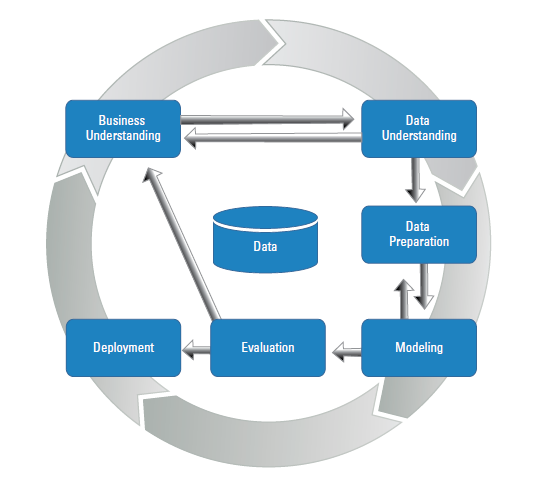
\includegraphics[scale=0.7]{Figure1.png}
	\caption{Predictive analytics process}
	\label{fig:Figure1}
\end{figure}
\newline
\subsubsection{Techniques available:}
From predictive analytics process, modeling and evaluation steps are where analysts use algorithms to produce key information they desire. Predictive modeling algorithms \cite{7} falls under Supervised Learning. In Supervised Learning, the predictor value or target variable is \textit{supervisor}, it is the column in dataset that is used for predicting value from other column values. It is divided into two sets:
\begin{enumerate}
	\item Classification: class based or discrete target variable
	\item Regression: continuous target variable 
\end{enumerate} 
Figure \ref{fig:Figure2} shows Predictive Analytics techniques used for modeling\cite{8}.
\begin{figure}[htbp]
	% center the image.
	\centering
	
	% include a png file. Adapt size to 0.5 * textwidth and retain aspect ratio (!)
	%	\resizebox{\textwidth}{!}{Figure1.png}}
	% NOTE: if possible do not include bitmap graphics in your paper, if available use
	% a vector graphics format
	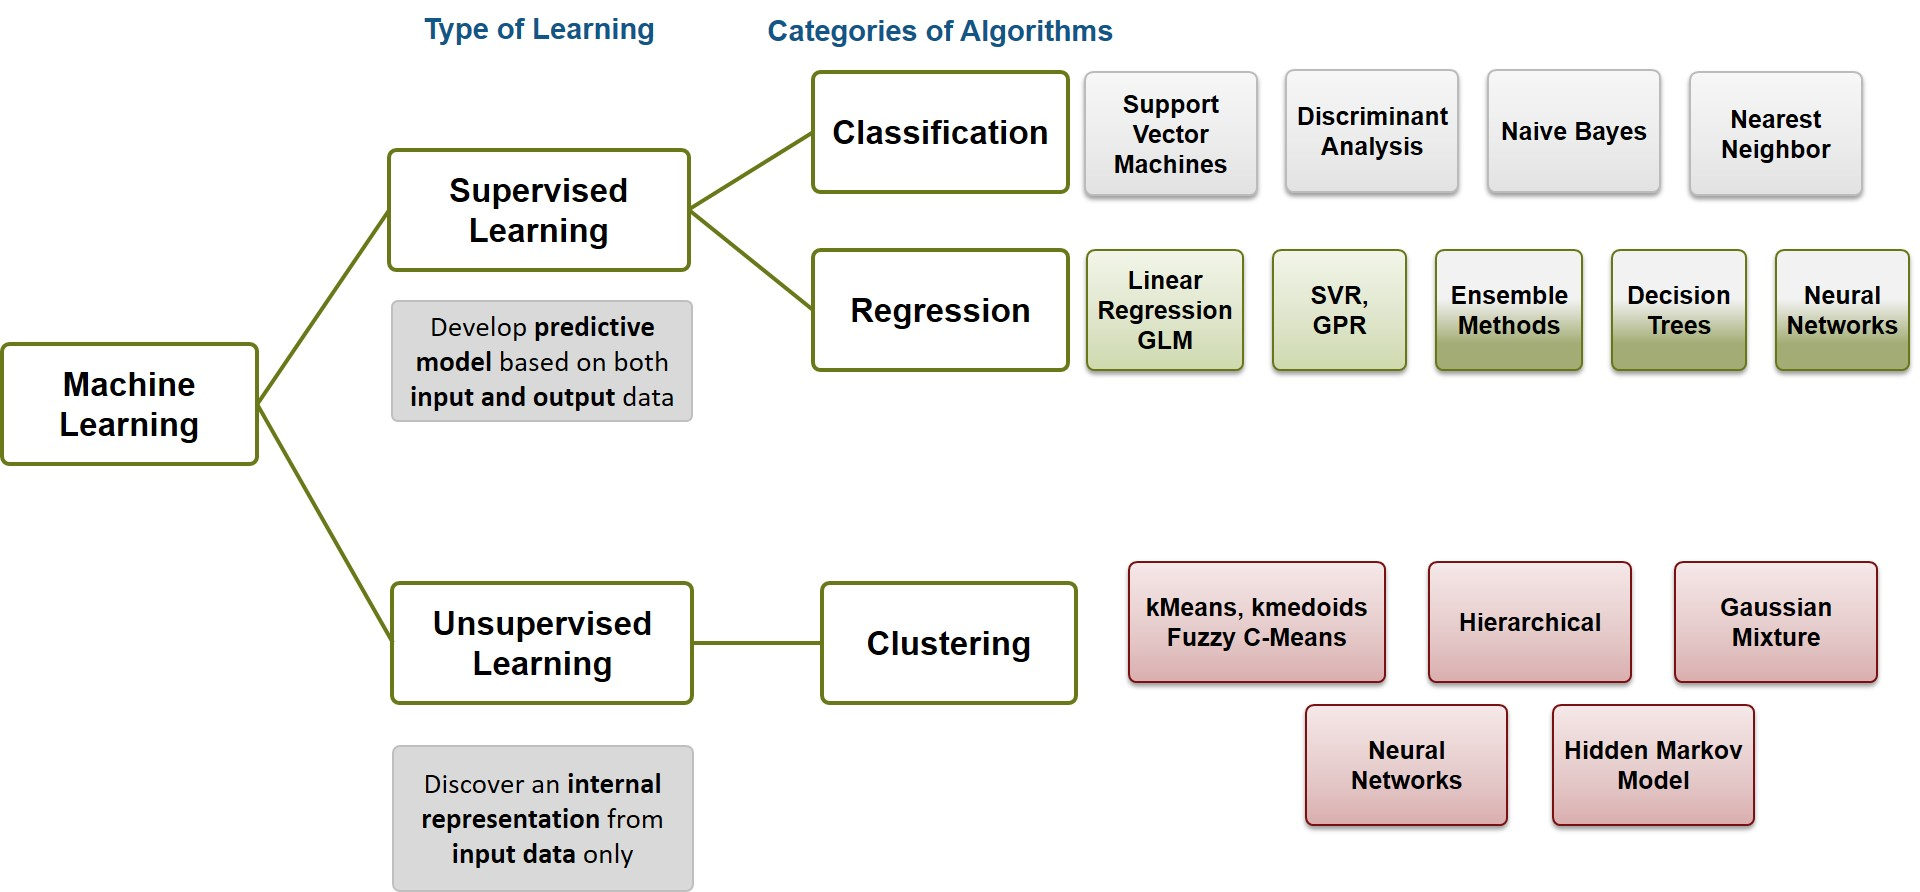
\includegraphics[scale=0.35]{Figure2.jpg}
	\caption{Predictive analytics techniques}
	\label{fig:Figure2}
\end{figure}

\vspace{-4mm}
\subsection{Predictive Analytics: Harness the power of Big Data}Almost every decision making process, be it in any enterprise, involves predictive analytics to drive their business better and helps gaining competitive edge in the market. Decision making in current era is based on day-to-day operational business data rather than on only special projects or scenario. Current tools and technologies are unsatisfactory and not up to standards to process such huge chunks of operational data. They are also unable to make in-depth insight and generate value. \newline
Thanks to Big Data technology and tools, predictive analytics can be applied to deluge of data at enterprise level, sometimes also called as Big Data Analytics. We have now many ways to tackle and test different predictive models at various level of framework for business strategies. Figure \ref{fig:Figure3} shows delineation of characteristics of Predictive Analytics techniques in transactional databases vs big data technologies. The former is based on prediction through historical structured data whereas big data platform can be used for modeling in real-time with structured, unstructured or semi-structured data. The common methods involved in transactional databases are data mining algorithms such as decision trees, regression, clustering, association rules, etc. In big data mediums, advanced techniques such as speech recognition, mobile based analytics, etc. [\cite{7}].\\
In the upcoming sections, we will be providing the conjunction of Predictive Analytics with Big Data technology and bring the following topics in coherence:\newline
(1) understanding big data architecture for analytical perspective \newline
(2) comparison and assessment of big data analytical tools used for predictions \newline
(3) address few of the challenges which collides interest of predictive analytics with big data. One of the key challenges being privacy- arising from ever increasing data from online services and personal devices such as mobile phones. These are subjected to risk of personal information being exposed for illicit uses. \newline
(4) discuss example from Enterprise Resource Planning (ERP) systems, and explore the opportunities of predictive analytics on ERP system's integrated big data hub. \newline
(5) discuss about Complex Event Processing which deals in identifying complex events based on the rules dictated by users of the system. In order to avoid the manual intervention of users for providing progressive rules, we will discuss about the framework that includes Predictive Analytics technologies in Complex Event Processing tools and applications. \newline
(6) case study demonstrating the power of predictive analytics coupled with big data technology.
\begin{figure}[htbp]
	% center the image.
	\centering
	\vspace{-0.85cm}
	% include a png file. Adapt size to 0.5 * textwidth and retain aspect ratio (!)
	%	\resizebox{\textwidth}{!}{Figure1.png}}
	% NOTE: if possible do not include bitmap graphics in your paper, if available use
	% a vector graphics format
	\hspace*{-0.45cm}
	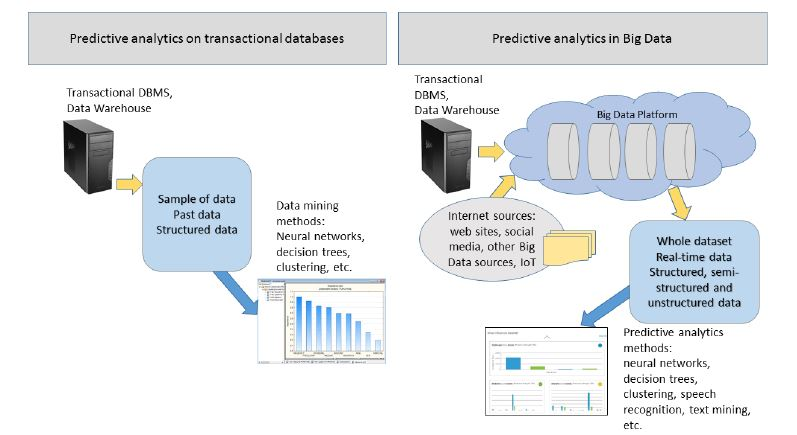
\includegraphics[scale=0.6]{Figure3.jpg}
	\caption{Predictive analytics in traditional databases vs Big Data}
	\label{fig:Figure3}
	\vspace{3.5cm}
\end{figure}
\section{Big Data System Architecture}

\subsection{Big Data Layered View}
\subsection{Big Data Value Chain View}

\section{Predictive Analytics Technologies}
\subsection{Big Data Platforms: Hadoop and Spark}
\subsection{Big Data Analytics Tools}
\subsection{Results: Comparison and Strategies}
\section{Issues in predictive analytics}
\subsection{Privacy challenges using Big Data analytics}
\subsection{Best practices available for preserving privacy}
\section{Example: Big Data Predictive Analytics in ERP Systems}
\section{Conceptual Framework: Predictive Complex Event Processing}
\subsection{Background}
\subsection{Exploiting the combined value of Complex Event Processing and Predictive Analytics}
\subsection{Conceptual CEP-PA framework}
\subsection{Proof of Concept}
\section{Case Study: Fraud Analytics}

\section{Conclusion}

\bibliographystyle{splncs} % other possible styles: plain, unsrt, abbrv, alpha
\bibliography{Example-Bib}

\end{document}
